\documentclass{article}
\usepackage[margin=1in]{geometry}
\usepackage{../common}
\usepackage{../pagesetup}

\begin{document}
%\lecture{**LECTURE-NUMBER**}{**DATE**}{**LECTURER**}{**SCRIBE**}
\lecture{21}{November 20}{Sasha Rush}{Raghu Dhara, Rui Fang}{Deep Learning in Health Care}%% Add your scribe names!!
We had a guest lecturer today: Sumit Chopra, head of AI Research at Imagen Technologies, a stealth-phase medical imaging startup.
\subsection{Past Work}
Before his work at Imagen, Dr. Chopra was a research scientist at Facebook AI Research. There, Dr. Chopra worked primarily in natural language processing (with Dr. Rush!). He completed his doctoral thesis under Yann LeCun at NYU. Here, he worked on Siamese Networks for picture distance metrics, DrLIM (dimensionality reduction by learning an invariant mapping) , and factor graphs for relational regression, a topic he then later applied at a startup to predict residential real estate prices. He has also worked at AT\&T labs as a research scientist.
\subsection{Computer Vision}

\subsubsection{Traditional Methods}
Traditional methods in computer vision perform image classification by transforming an input image into features through a hand-crafted feature extractor (SIFT, HOG, ...) and then classifying the features using a classifier (SVMs, Neural Network (rarely), ...). The drawback of such methods is that hand crating features become challenging when input is not visually perceptible: depth map, etc. 

\subsubsection{Deep Learning: Convolutional Neural Networks (CNNs)}

Unlike traditional methods, deep learning proposes to learn the features from scratch - learn everything end to end. The intuition behind deep learning is to learn a highly complex function composed of lots of simple functions, of which the parameters will be learned. The main class of deep learning architectures used in computer vision is the convolutional neural networks. 

There are three basic types of hidden layers in a CNN: convolutional layer, non-linearity layer, and pooling layer. 

\begin{itemize}
    \item The convolutional layer is built upon convolution operation, which applies a kernel matrix to an input matrix and returns the dot products between the kernel and each receptive field. For example, Figure \ref{fig:convolution} shows applying a $3\times 3$ kernal with stride $=1$ (move one pixel at a time) over a $7\times7$ input matrix results in a $5\times5$ output matrix. 

    \item The non-linearity layer applies a non-linear activation function to the output of the convolutional layer. 
    
    \item The pooling layer works as subsampling: it applies a kernel (usually a max function) to an input matrix without overlapping, as shown in Figure \ref{fig:pooling}. The pooling layer reduces spatial dimension of the input and results in spatial invariance. 
\end{itemize}

A typical CNN architecture is shown in Figure \ref{fig:cnn}. This CNN performs an image level classification - it takes the entire image and output predictions of the major theme of this image. The input image is convoluted and subsampled a few times before getting classified through the fully connected layers.   


\begin{figure}
    \centering
    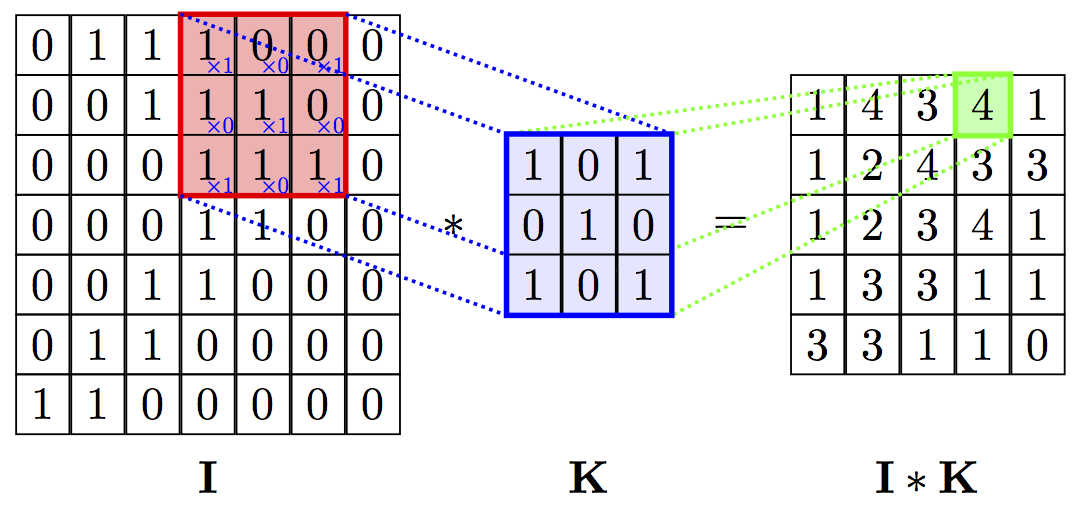
\includegraphics[width=0.5\textwidth]{21/convolution.png}
    \caption{Convolution}
    \label{fig:convolution}
\end{figure}

\begin{figure}
    \centering
    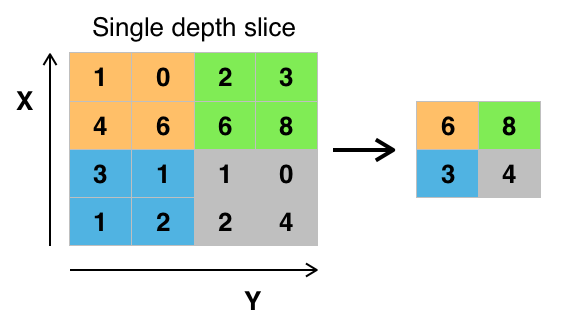
\includegraphics[width=0.5\textwidth]{21/pooling.png}
    \caption{Pooling}
    \label{fig:pooling}
\end{figure}

\begin{figure}
    \centering
    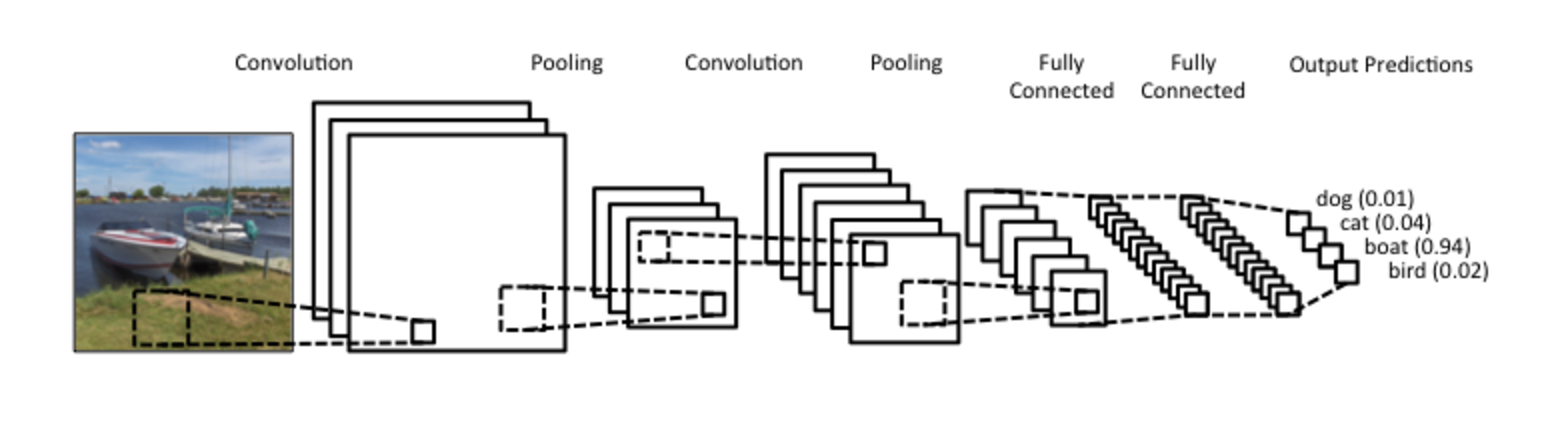
\includegraphics[width=0.9\textwidth]{21/cnn.png}
    \caption{Typical CNN architecture}
    \label{fig:cnn}
\end{figure}

\subsubsection{Pixel Level Classification CNNs}

For image recognition, the tasks range from image level classification to object level classification to pixel level classification. The focus here is pixel level classification: the convolutional neural networks have a loss function associated with every pixel. Applications of pixel level classification include scene understanding, semantic segmentation, depth map prediction, medical imaging, etc.  

We introduce three CNN based architectures in this category: 

\begin{enumerate}

\item Fully Convolutional Network (FCN) \footnote{Long et al., \textit{Fully Convolutional Networks for Semantic Segmentation}}

Fully convolutional networks take input of arbitrary size and produce correspondingly sized output (see Figure \ref{fig:fcn}). Different from typical classification CNN architectures where outputs are non-spatial, in FCN the classification layers (fully-connected layers) are viewed as convolutions with kernels that cover their entire input regions, therefore generating 2D classification maps as outputs (see Figure \ref{fig:fcn_classifier}). While the output is 2D, it is still coarse due to subsampling. Hence, upsampling is needed to generate outputs of the same size as inputs. In addition, the networks are designed to combine predictions from both the final layer and the intermediate layer to provide finer details (see Figure \ref{fig:fcn_upsample} and Figure \ref{fig:fcn_results}).  

\begin{figure}[h]
    \centering
    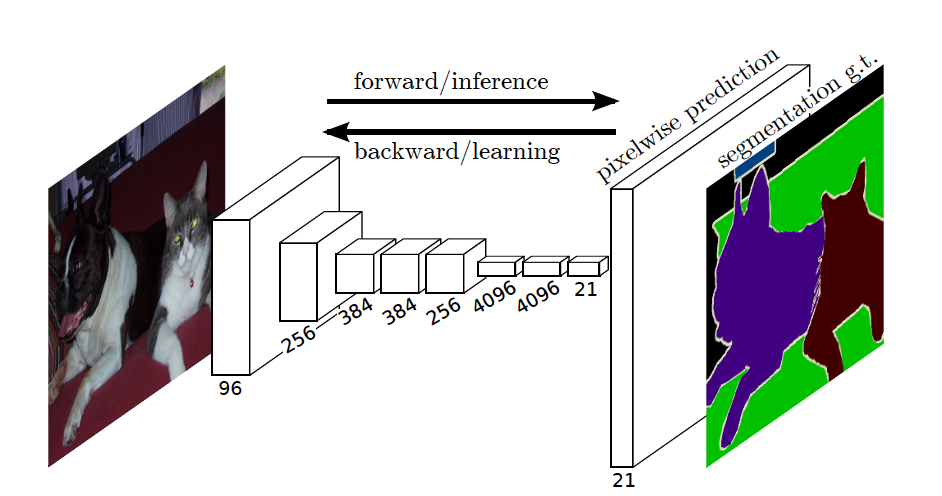
\includegraphics[width=0.5\textwidth]{21/fcn.png}
    \caption{Fully convolutional networks can efficiently learn to
make dense predictions for per-pixel tasks like semantic segmentation.}
    \label{fig:fcn}
\end{figure}

\begin{figure}[h]
    \centering
    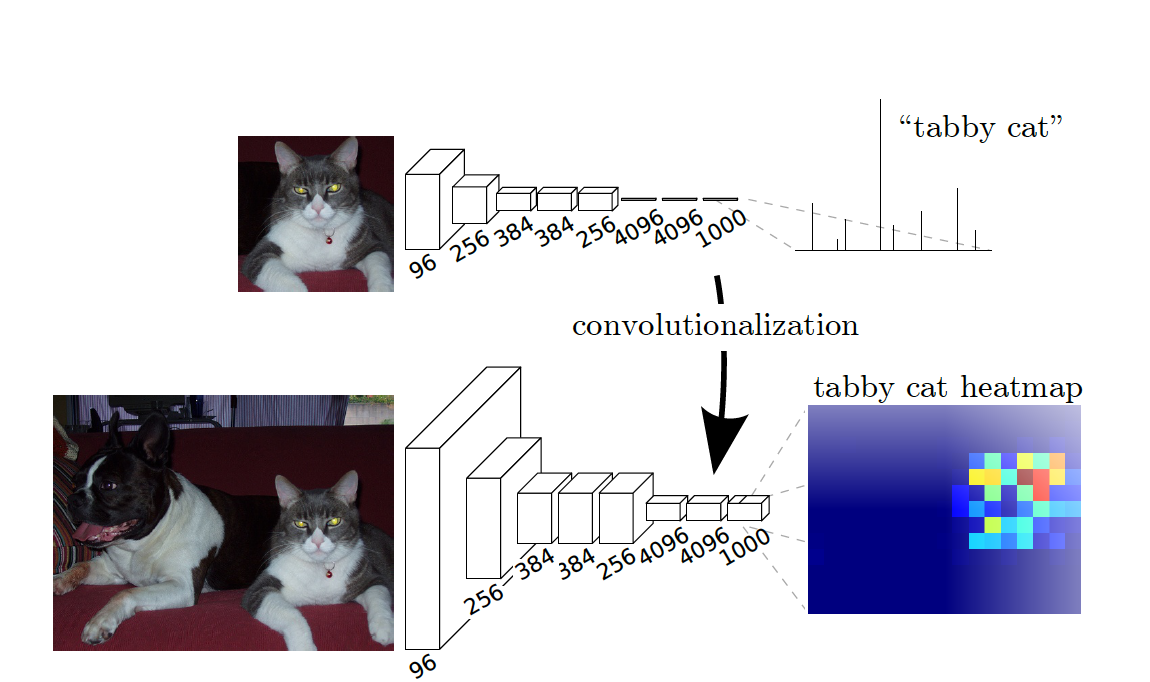
\includegraphics[width=0.6\textwidth]{21/fcn_classifier.png}
    \caption{Transforming fully connected layers into convolution
layers enables a classification net to output a heatmap.}
    \label{fig:fcn_classifier}
\end{figure}

\begin{figure}[h]
    \centering
    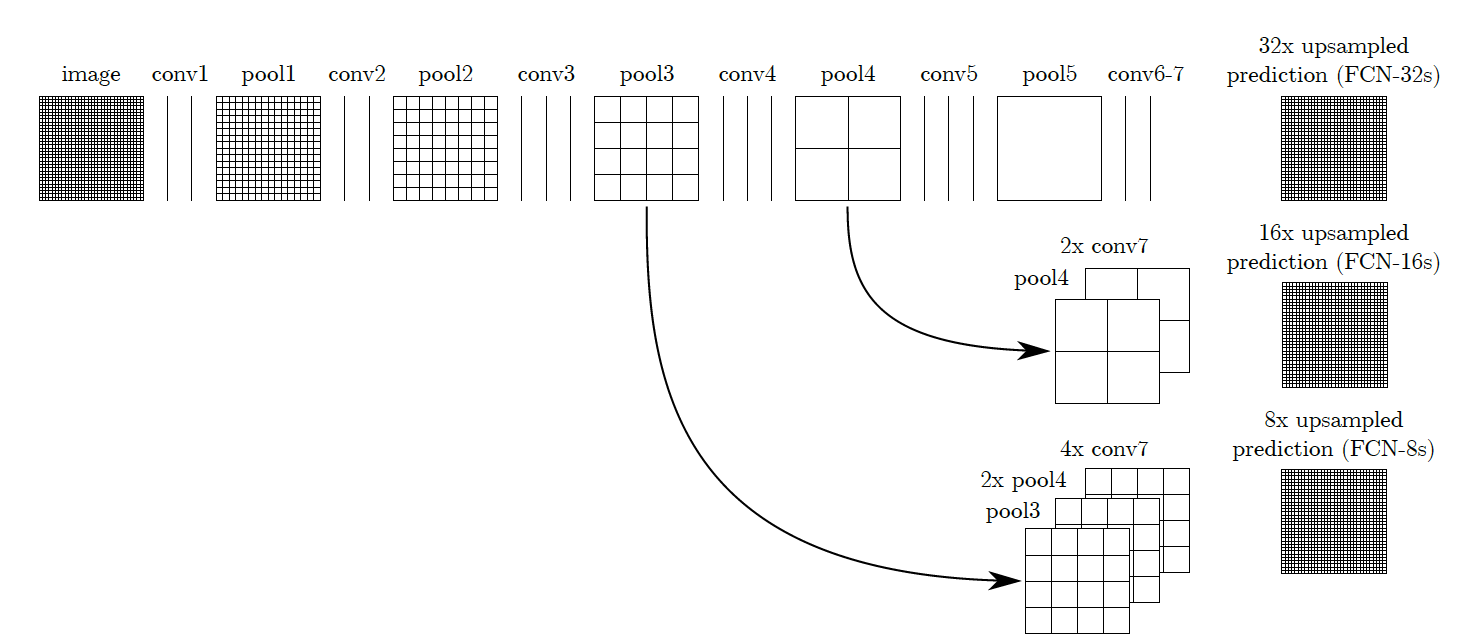
\includegraphics[width=0.9\textwidth]{21/fcn_upsample.png}
    \caption{A fully convolutional net (FCN) for segmentation
that combines layers of the feature hierarchy and
refines the spatial precision of the output.}
    \label{fig:fcn_upsample}
\end{figure}

\begin{figure}[h]
    \centering
    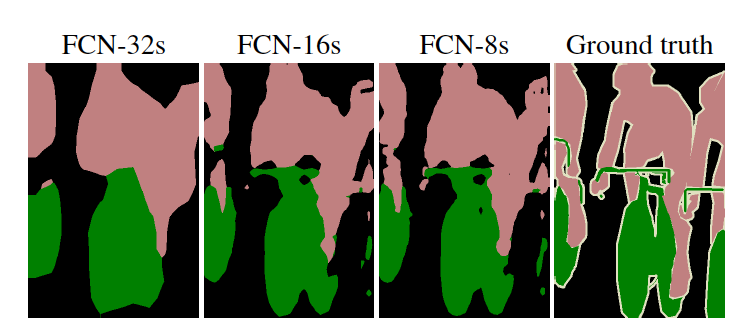
\includegraphics[width=0.6\textwidth]{21/fcn_results.png}
    \caption{Refining fully convolutional nets by fusing information from layers with different strides improves segmentation detail.}
    \label{fig:fcn_results}
\end{figure}



\item U-Net \footnote{Ronneberger et al., \textit{U-Net: Convolutional Networks for Biomedical
Image Segmentation}}

Since annotated examples are not as easily obtainable for biomedical tasks due to the significant and specialized effort required to procure them, U-Nets tries to use the provided samples efficiently. The architecture consists of a contracting path to capture
context and a symmetric expanding path that enables precise localization (see Figure \ref{fig:U-net}).
The contracting path involves repeatedly applying the following sequence: a 3x3 convolution, a ReLU, and a 2x2 max pool. The expansive step involves repeatedly applying the following sequence: upsampling the feature map followed by a 2x2 convolution (``"up-convolution"), a concatenation of the corresponding feature map from the contracting path, another 3x3 convolution, and a ReLU. At the final layer a 1x1 convolution is used to map each 64- component feature vector to the desired number of classes, for a total of 23 convolutional layers.


For training, the energy function is computed by a pixel-wise soft-max over the final
feature map combined with the cross entropy loss function that penalizes deviation from the ground truth pixel labels (see Figure \ref{fig:unet_training}). These U-Nets train and run faster than the previous state-of-the art deep convolutional networks that came before it (10 hours to train, under a second to run), making them a compelling option. They are invariant to elastic deformations to the input image, a strategy that was leveraged to augment the data.


\begin{figure}[h]
    \centering
    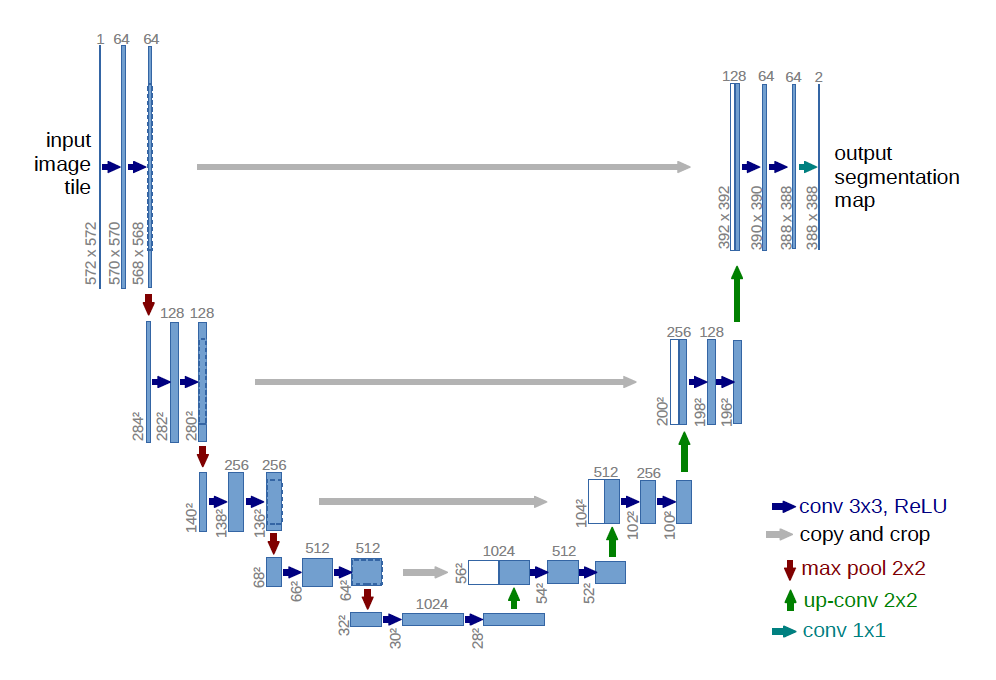
\includegraphics[width=0.8\textwidth]{21/unet.png}
    \caption{U-net architecture. Notice the namesake U shape.}
    \label{fig:U-net}
\end{figure}


\begin{figure}[h]
    \centering
    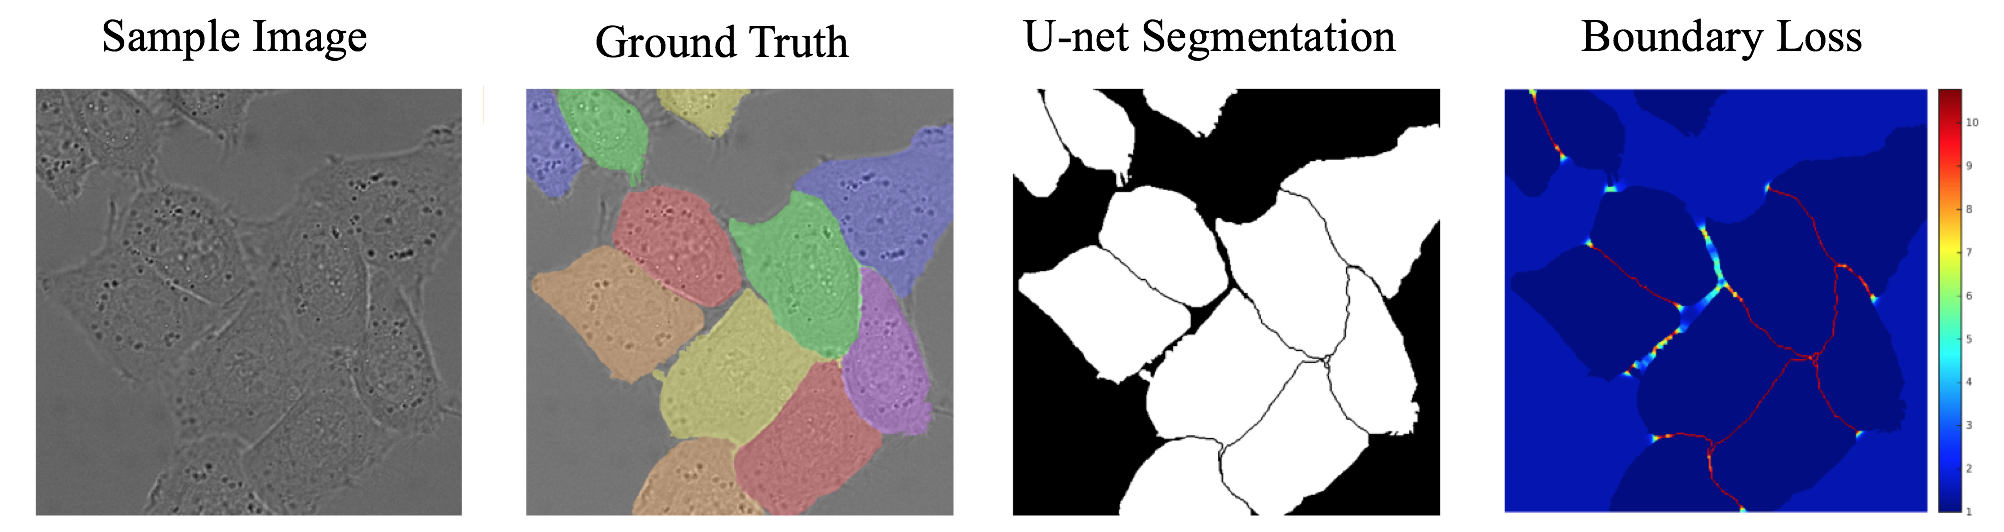
\includegraphics[width=0.8\textwidth]{21/unet_borders.png}
    \caption{U-Net producing a pixel-wise loss map to force the network to learn border pixels}
    \label{fig:unet_training}
\end{figure}




\begin{figure}[!]
    \centering
    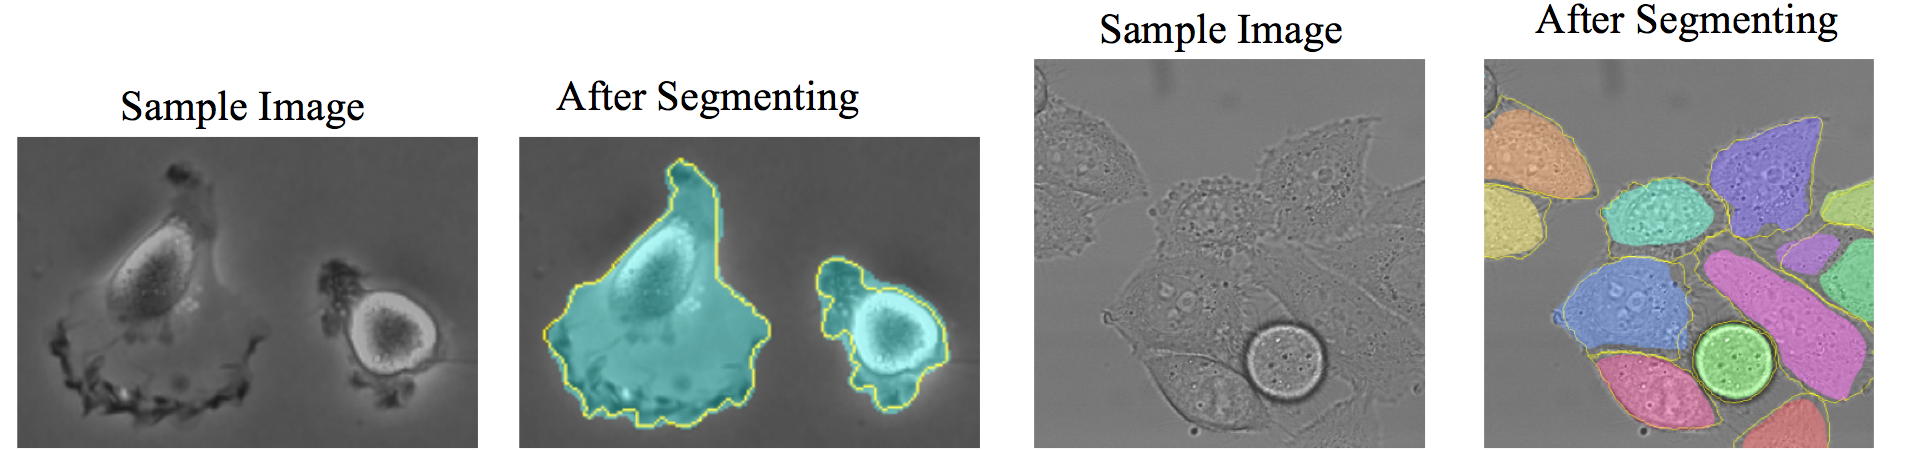
\includegraphics[width=0.8\textwidth]{21/unet_results.png}
    \caption{Example segmentation results with U-Net. The yellow border is the ground truth.}
    \label{fig:unet_results}
\end{figure}





\item Atrous (Dilated) Convolution \footnote{Chen et al., \textit{DeepLab: Semantic Image Segmentation with Deep Convolutional Nets, Atrous Convolution,
and Fully Connected CRFs}}

Atrous convolution is convolution with upsampled filters. This allows us to explicitly control the resolution at which feature responses are computed within deep CNNs. Such an ability gives us a clear advantage: the output image will be closer in size to the input image, enabling sharper decision boundaries at useful scales. Traditional methods often involve downsampling steps that produce outputs significantly smaller than the inputs, and the corrective upsampling introduces pixel declocalization. To mitigate this, atrous convolutional networks combine the results at the final layer of a deep convolutional neural network with a fully connected Conditional Random Field (CRF), which is shown both qualitatively and quantitatively to improve localization performance. 

\begin{figure}[h]
    \centering
    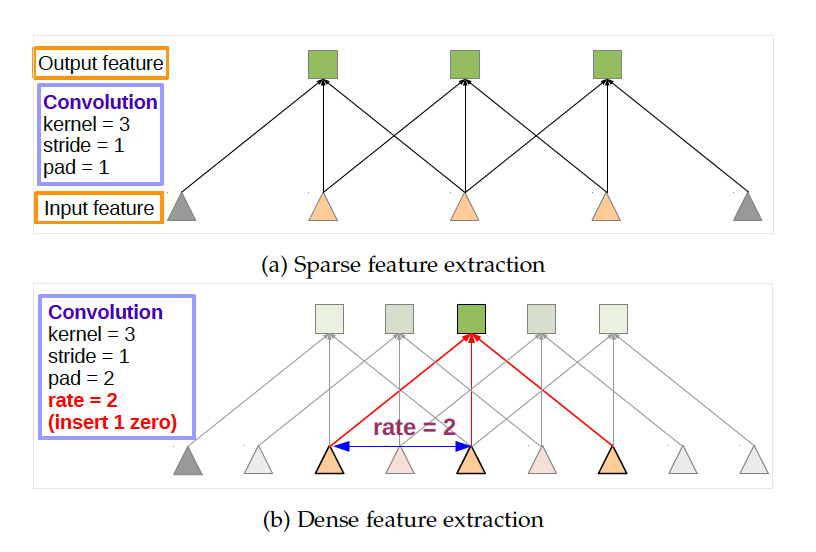
\includegraphics[width=0.5\textwidth]{21/deeplab.png}
    \caption{Atrous convolution in 1D}
    \label{fig:atrous}
\end{figure}


\begin{figure}[h]
    \centering
    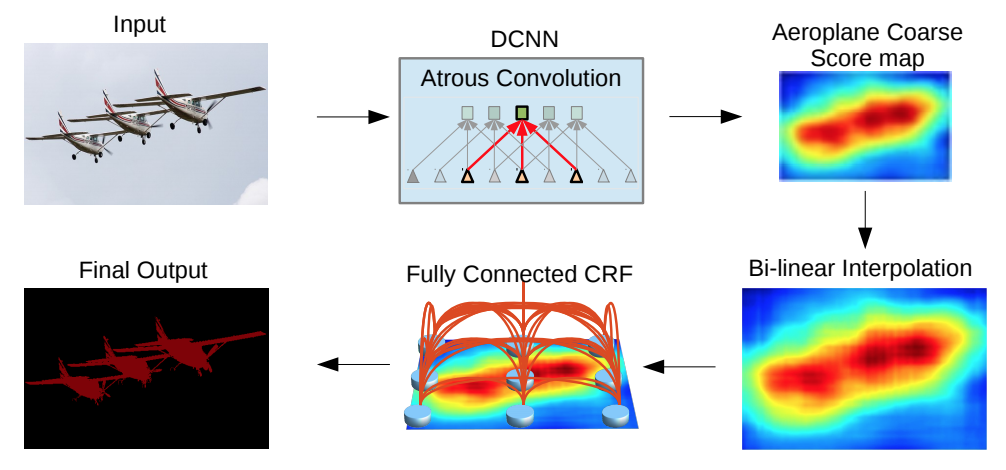
\includegraphics[width=0.5\textwidth]{21/atrous_overview.png}
    \caption{Overall procedure for atrous convolution}
    \label{fig:atrous_sketch}
\end{figure}



\begin{figure}[h]
    \centering
    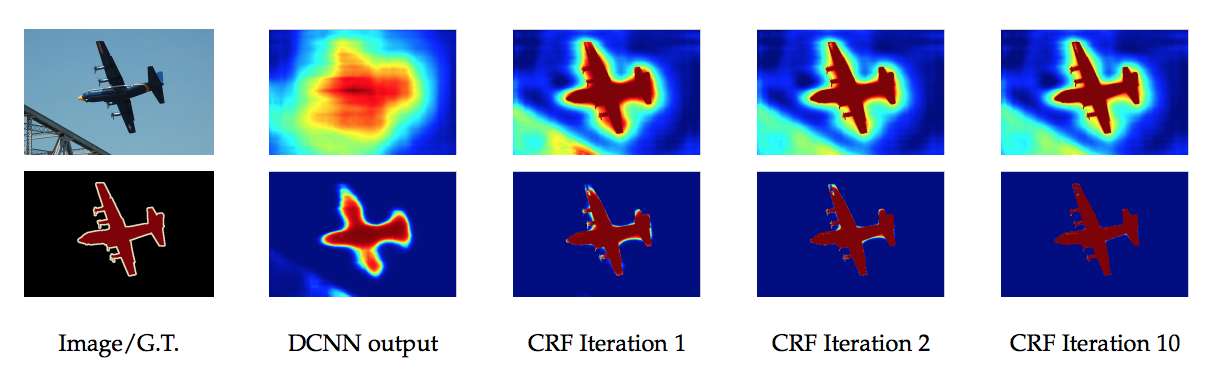
\includegraphics[width=0.5\textwidth]{21/crf_iter.png}
    \caption{Repeated mean-field iterations further refine the score maps (top row) and belief maps (bottom row)}
    \label{fig:atrous_iter}
\end{figure}



\end{enumerate}



\subsection{Healthcare Data Landscape and Diagnostic Radiology}
\subsubsection{Providers and Payers}
In general, medical data is difficult to acquire. There are two primary repositories: healthcare providers and payers. Providers such as hospitals are often secretive about their datasets, which are often incomplete. Payers such as insurance companies have more thorough datasets so long as the patient does not change insurers. Medicare data is somewhat perpetual as well but is biased towards older people.

\subsubsection{Why Diagnostic Radiology is Important}
\begin{enumerate}
    \item Prevalence of studies: 600 million per year in the US, over 5 billion per year in the world
    \item Shortage of skilled radiologists: 11,000 fewer than needed in the US, some countries only have a couple in total
    \item Prevalence of errors: 5-15\% error rate in the US, which has a very sophisticated medical system - this translates to 30-90 million misdiagnoses per year, a number of which are potentially fatal
\end{enumerate}

\subsubsection{AI in Diagnostic Radiology}
Given an image along with possibly other modalities of data, the principal goals are to
\begin{enumerate}
    \item Identify the region(s) of interest/anomaly
    \item Infer whether the image has a clinically relevant medical condition
    \item Infer the underlying cause of the condition (causal inference)
    \item Write the full diagnostic report
\end{enumerate}

\end{document}

